\documentclass[exercice]{thedocument}%
\usepackage{tkz-euclide}%
\startdatakeys
\source{}
\BO{2026}
\cycle{4}
\competencesDuSocle{CA}
\objectifsApprentissage{C4B1ba,C4C1aa,C4B2db}
\automatismes{C4B1da,C4B1eb}
\enddatakeys
\begin{document}%
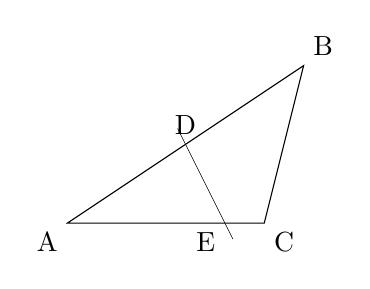
\begin{tikzpicture}
    \coordinate[label=below left:A](A)at(0,0);
    \coordinate[label=below left:E](E)at(2,0);
    \coordinate[label=below right:C](C)at(2.5,0);
    \coordinate[label=above right:B](B)at(3,2);
    \path(A)--(B)coordinate[pos=0.5,label=above:D](D);
    \draw(A)--(C)--(B)--cycle;
    \tkzDrawLine(D,E)
\end{tikzpicture}
\begin{enumerate}
    \item À vue d'\oe il, préciser pour chacun des angles suivants s'il est
    aigu, obtus ou droit :
    $$\widehat{\text{BAC}}\hskip20pt\widehat{\text{ADE}}\hskip20pt\widehat{\text{ABE}}
    \hskip20pt\widehat{\text{BEC}}\hskip20pt\widehat{\text{ACB}}
    $$
    \item Mesurer chacun des angles avec le rapporteur et vérifier les
    réponses données à la question {\bfseries 1)}.
\end{enumerate}
\end{document}
